\documentclass{beamer}

\usepackage{graphicx}       % Extended support for \includegraphics
\usepackage{tikz}           % Powerful drawing package, part of pgf
\usepackage{hyperref}       % \url command for decent line breaks in urls
\usepackage{array}          % Improved array support
\usepackage{textcomp}       % Extra symbols
\usepackage{listings}       % Source code listings
\usepackage{xcolor}         % Syntax colouring support


% Listing defaults configuration
\lstset{
    keywordstyle=\bfseries\color{blue},
    commentstyle=\itshape\color{green!50!black},
    stringstyle=\color{red!60!black},
    numberstyle=\color{gray},
    basicstyle=\footnotesize\ttfamily,
    showstringspaces=false,
    frame=single,
}


\usetheme{dlstalk}
\setbeamertemplate{navigation symbols}{}
\setbeamertemplate{items}[circle]

\hyphenpenalty 4000 \sloppy

\title[Python Soft IOC]{The Python Soft IOC}
\author{Michael Abbott}
\date{18th February 2015}

\begin{document}


% ------------------------------------------------------------------------------
%
\begin{frame}\frametitle{Forthcoming Controls Seminars}

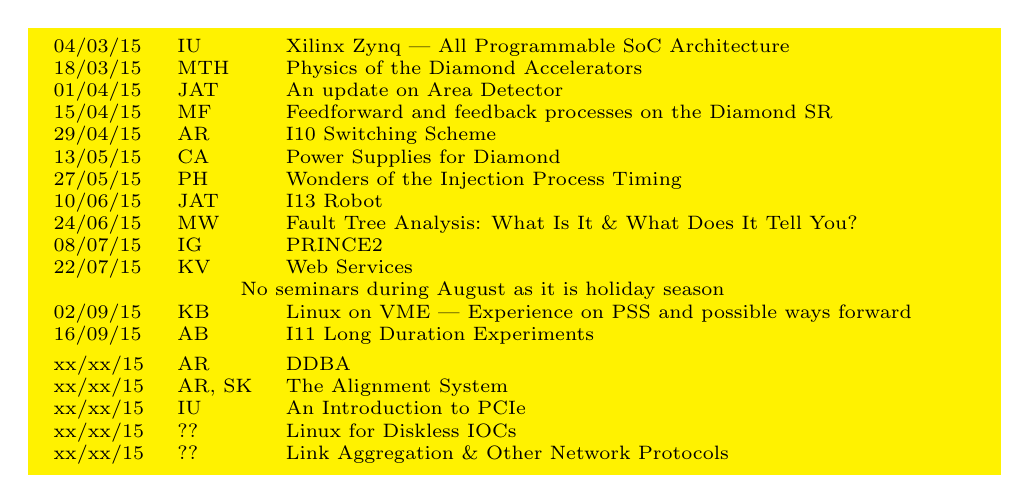
\begin{tikzpicture}
\node [fill=yellow] {
\scriptsize
\begin{tabular*}{\textwidth}{lll}
04/03/15 & IU &  Xilinx Zynq --- All Programmable SoC Architecture \\
18/03/15 & MTH & Physics of the Diamond Accelerators \\
01/04/15 & JAT & An update on Area Detector \\
15/04/15 & MF &  Feedforward and feedback processes on the Diamond SR \\
29/04/15 & AR &  I10 Switching Scheme \\
13/05/15 & CA &  Power Supplies for Diamond \\
27/05/15 & PH &  Wonders of the Injection Process Timing  \\
10/06/15 & JAT & I13 Robot \\
24/06/15 & MW &  Fault Tree Analysis: What Is It \& What Does It Tell You?  \\
08/07/15 & IG &  PRINCE2 \\
22/07/15 & KV &  Web Services \\
\multicolumn{3}{c}{No seminars during August as it is holiday season} \\
02/09/15 & KB &  Linux on VME --- Experience on PSS and possible ways forward \\
16/09/15 & AB &  I11 Long Duration Experiments \\[1ex]
xx/xx/15 & AR &  DDBA \\
xx/xx/15 & AR, SK & The Alignment System \\
xx/xx/15 & IU &  An Introduction to PCIe \\
xx/xx/15 & ?? &  Linux for Diskless IOCs \\
xx/xx/15 & ?? &  Link Aggregation \& Other Network Protocols \\
\end{tabular*}
};
\end{tikzpicture}

\begin{footnotesize}
\color{red}
Volunteers to present future seminars from September 2015 are needed.

\color{blue}
Please contact James O'Hea or Mark Heron with a proposed topic.
\end{footnotesize}

\end{frame}


% ------------------------------------------------------------------------------
%
\begin{frame}
\titlepage
\end{frame}

% Place date discreetely on every slide.
\setbeamertemplate{footline}{\hspace*{\fill}\insertdate}


% ------------------------------------------------------------------------------
%
\begin{frame}{Python Soft IOC: Introduction}

The Python Soft IOC is a tool to make it easy to create EPICS IOCs with no
hardware support using Python.

\medskip

This tool consists of the following components:

\begin{itemize}
\item An EPICS IOC executable
\item An integrated Python interpreter
\item A Python library to assist in dynamically building and running an IOC
\end{itemize}

\end{frame}


% ------------------------------------------------------------------------------
%
\begin{frame}{Examples of Python Soft IOCs}

This tool is used by a number of Diagnostics IOCs:

\begin{description}
\item[Concentrator]
The Diagnostics concentrator gathers updates from BPMs around the ring into
waveforms.
\item[Slow Feedback]
Complex control loops running at around 1\,Hz are perfect for implementation in
Python.
\item[Postmortem Servers]
Here the IOC part is really only used to identify the machine.
\item[Spectrum Analyser]
This server digests Fast Archiver data and generates thousands (literally) of
long waveforms containing power spectra data.
\end{description}

Also used by Nick Battam for test PVs.

\end{frame}


% ------------------------------------------------------------------------------
%
\begin{frame}{Demonstration}
\end{frame}


% ------------------------------------------------------------------------------
%
\begin{frame}{Creating a Python Soft IOC}
The software framework requires the following steps:

\begin{itemize}
\item A wrapper shell script
\item Boilerplate DLS versioning and \texttt{import} statements
\item PV creation and initialisation
\item IOC startup boilerplate (two library calls)
\item IOC background activity startup (optional)
\item Dwell at interactive shell (optional)
\end{itemize}

\end{frame}


% ------------------------------------------------------------------------------
%
\begin{frame}[fragile]\frametitle{Startup Script}

A startup shell script is needed to launch the IOC.

\medskip

I suggest naming the following script \texttt{start-ioc}, then this can be used
to launch the IOC.  Note the versioning in this file.

\lstset{language=bash}
\begin{lstlisting}
#!/bin/sh

EPICS_VERSION=R3.14.12.3
PYIOC_VERSION=2-8
PYIOC=/dls_sw/prod/$EPICS_VERSION/support/pythonSoftIoc/\
$PYIOC_VERSION/pythonIoc

cd "$(dirname "$0")"
exec $PYIOC example_ioc.py "$@"
\end{lstlisting}

\end{frame}


% ------------------------------------------------------------------------------
%
\begin{frame}[fragile]\frametitle{Versioning Boilerplate}

Mostly all too familiar Python versioning boilerplate goes at the start of the
top level file:

\lstset{language=Python}
\begin{lstlisting}
# DLS versioning boilerplate
from pkg_resources import require
require('numpy==1.7.0')
require('cothread==2.12')
require('iocbuilder==3.50')

# Python Soft IOC framework components
from softioc import softioc, builder
import cothread
\end{lstlisting}

\end{frame}


% ------------------------------------------------------------------------------
%
\begin{frame}[fragile]\frametitle{Simple Example}

A minimal Python soft IOC showing PV creation, startup, shell.

% \lstinputlisting[language=Python]{minimal.py}
\lstset{language=Python}
\begin{lstlisting}
# Create a PV
builder.SetDeviceName('TS-XX-TIME-01')
time_pv = builder.aIn('TIME', DESC = 'Unix timestamp')

# Fire up the IOC.  No PV creation possible past this point!
builder.LoadDatabase()
softioc.iocInit()

# Create timer to update the PV: generate updates
import time
def update_time():
    time_pv.set(time.time())
cothread.Timer(1, update_time, retrigger=True)

# Sit and wait with an interactive shell
softioc.interactive_ioc(globals())
\end{lstlisting}

\end{frame}


% ------------------------------------------------------------------------------
%
\begin{frame}{Simple Example Explained}
\begin{itemize}
\item All PVs need to be named and defined before the IOC database can be
loaded.
\item Once the database has been loaded then the IOC is started by calling
\texttt{iocInit}.
\item Past this point no further records can be created.
\item By default all In records are created with \texttt{I/O Intr} scanning, so
updates are generated internally.
\end{itemize}
\end{frame}


% ------------------------------------------------------------------------------
%
\begin{frame}{IOC Shell}
The shell launched by \texttt{softioc.interactive\_ioc()} is the Python
interpreter with a number of EPICS commands added to the working environment,
including:

\begin{ttfamily}
\begin{quote}
dba, dbl, dbnr, dbgrep, dbgf, dbpf, dbpr, dbtr, dbior, scanppl, scanpel,
scanpiol, generalTimeReport, eltc
\end{quote}
\end{ttfamily}

plus quite a few others I added but don't have descriptions for.  That's a
pretty obscure list of commands!

\end{frame}


% ------------------------------------------------------------------------------
%
\begin{frame}[fragile]\frametitle{Creating PVs}

All PV creation functions are in the \texttt{softioc.builder} module.

\medskip

First set the name prefix by calling \texttt{SetDeviceName()}, eg:

\lstset{language=Python}
\begin{lstlisting}
SetDeviceName('TS-XX-TIME-01')
\end{lstlisting}

Then PVs can be created by the following functions:

\begin{quote}
\texttt{aIn()}, \texttt{aOut()}, \texttt{boolIn()}, \texttt{boolOut()},
\texttt{longIn()}, \texttt{longOut()}, \texttt{stringIn()},
\texttt{stringOut()}, \texttt{mbbIn()}, \texttt{mbbOut()}, \texttt{Waveform()},
\texttt{WaveformOut()}.
\end{quote}

For example, calling \texttt{aIn('VALUE')} will now create an \texttt{ai} record
called \texttt{TS-XX-TIME-01:VALUE}.

\end{frame}


% ------------------------------------------------------------------------------
%
\begin{frame}{Record Creation}

All the record creation functions have a common form:

\begin{itemize}
\item They all return a record object which supports at least two methods:
\texttt{.set()} and \texttt{.get()} to manage the value.
\item The first argument is used to name the record, together with the currently
set prefix.
\item A number of optional arguments have function specific functions, for
example the range of values for an \texttt{ai} record can be specified.
\item The named argument \texttt{initial\_value} can specify the initial value
for any record.
\item Out and Waveform records support further named arguments.
\item The remaining named arguments can be used to specify a value for any EPICS
database field.
\end{itemize}

\end{frame}


% ------------------------------------------------------------------------------
%
\begin{frame}[fragile]\frametitle{Record Creation Example}

For example:

\lstset{language=Python}
\begin{lstlisting}
rec_in = aIn('VALUE', 0, 10,
    initial_value = 0.1,
    EGU = 'V', DESC = 'A record of some sort')

rec_out = aOut('VALOUT', 0, 100,
    initial_value = 0.3, on_update = update_rec_out,
    EGU = '%', DESC = 'An output control')
\end{lstlisting}

In this example \texttt{update\_rec\_out(new\_value)} will be called each time a
CA put to the \texttt{VALOUT} record occurs.


\end{frame}


% ------------------------------------------------------------------------------
%
\begin{frame}{Basic Record Types}

There are two classes of record, input and output, together with five
fundamental datatypes; waveforms are a third record class supporting its
own set of datatypes, which can be created as In or Out records.

\medskip

\begin{center}
\begin{tabular}{l|c|c|}
Datatype & In & Out \\
\hline
Double & \texttt{ai} & \texttt{ao} \\
Integer & \texttt{longin} & \texttt{longout} \\
Boolean & \texttt{bi} & \texttt{bo} \\
String & \texttt{stringin} & \texttt{stringout} \\
Enum & \texttt{mbbi} & \texttt{mbbo} \\
Waveform & \multicolumn{2}{c|}{\texttt{waveform}} \\
\hline
\end{tabular}
\end{center}

\end{frame}


% ------------------------------------------------------------------------------
%
\begin{frame}{Special Record Arguments}

Each record type supports a different set of anonymous arguments.

\begin{description}
\item[aIn, aOut] Lower and upper range.
\item[boolIn, boolOut] Strings for 0 and 1 values.
\item[longIn, longOut] Lower and upper range, and engineering
units\footnotemark.
\item[stringIn, stringOut] No unnamed arguments.
\item[mbbIn, mbbOut] Complicated!  At its simplest, a list of names for
enumeration strings, but can be a list of tuples.
\item[Waveform, WaveformOut] An initial value can be passed as the only
anonymous argument.
\end{description}

\footnotetext[1]{Inconsistent with \texttt{aIn}, \texttt{aOut}, this is probably
a bug.}

\end{frame}


% ------------------------------------------------------------------------------
%
\begin{frame}{In Records}

In records are created with the appropriate call to one of:

\begin{quote}
\texttt{aIn()}, \texttt{boolIn()}, \texttt{longIn()}, \texttt{stringIn()},
\texttt{mbbIn()}, \texttt{Waveform()}
\end{quote}

You'll want to hang onto the returned value so that you can update it when
appropriate with one of these methods:

\begin{description}
\item[.set(value [,severity, ...{]})]
Updates value and (by default) forces record to process.
\item[.set\_alarm(severity [, ...{]})]
Sets alarm severity without changing the value, updates record.
\item[.get()]
Returns current value associated with record.
\end{description}

\end{frame}


% ------------------------------------------------------------------------------
%
\begin{frame}[fragile]\frametitle{In Record Example}

\lstset{language=Python}
\begin{lstlisting}
class Example:
    def __init__(self):
        self.pv = aIn('PV', 0, 100, EGU = '%',
            DESC = 'Some description that makes sense')

    def do_update(self, new_value):
        self.pv.set(new_value)
\end{lstlisting}

Arrange to create \texttt{Example} during IOC startup, arrange for the
\texttt{do\_update} method to be called when appropriate.

\end{frame}


% ------------------------------------------------------------------------------
%
\begin{frame}{Out Records}

Out records are created with the appropriate call to one of:

\begin{quote}
\texttt{aOut()}, \texttt{boolOut()}, \texttt{longOut()}, \texttt{stringOut()},
\texttt{mbbOut()}, \texttt{WaveformOut()}
\end{quote}

Either hang onto the result so its value can be interrogated with the
\texttt{.get()} method, or configure an \texttt{on\_update} callback.

\end{frame}


% ------------------------------------------------------------------------------
%
\begin{frame}{Out Record Named Arguments}

Because Out records can be written to from the outside a little more control is
needed over their behaviour.  The following optional keyword arguments are
available:

\begin{description}
\item[on\_update(value)]
This is called via cothread after record process has completed to notify an
incoming value.
\item[always\_update]
By default a record update is ignored if it doesn't change the record value;
setting this flag changes this behaviour.
\end{description}

\end{frame}


% ------------------------------------------------------------------------------
%
\begin{frame}{Waveform Records}

There are two methods for creating \texttt{waveform} records:
\texttt{Waveform()} for In records and \texttt{WaveformOut()} for Out records.

\medskip

For waveforms some selection of the following arguments must be specified:

\begin{description}
\item[initial\_value]
This can be an anonymous argument, waveform length and type are computed
from this value.
\item[length] Number of elements in waveform if no initial value.
\item[datatype] Datatype as a Python class if no initial value.
\item[FTVL] An alternative to datatype.
\end{description}

\medskip

For \texttt{WaveformOut} the usual Out arguments are available.

\end{frame}


% ------------------------------------------------------------------------------
%
\begin{frame}{Python Soft IOC and Support Modules}

The Python Soft IOC is statically linked, so it can only use these built-in
support modules:

\begin{description}
\item[devIocStats]
A function \texttt{softioc.devIocStats} implements support for this.
\item[PV logging]
Importing \texttt{softioc.pvlog} is enough to implement logging of all CA puts.
\end{description}

\medskip

Python Soft IOC really isn't designed for hardware support or for integrating
existing support modules.  If you want to use a support module you don't want
Python Soft IOC!

\end{frame}


% ------------------------------------------------------------------------------
%
\begin{frame}{Autosave/Restore}

This functionality is missing.  This omission may be a mistake, I'm not
altogether sure \dots

\end{frame}


% ------------------------------------------------------------------------------
%
\begin{frame}{Python Soft IOC Internals}

The Python Soft IOC is constructed from these components:

\begin{itemize}
\item EPICS IOC
\item Python Interpreter
\item Cothread
\item IOC Builder
\end{itemize}

\end{frame}


% ------------------------------------------------------------------------------
%
\begin{frame}[fragile]\frametitle{EPICS IOC and Python Interpreter}

The core Python Soft IOC executable is extremely simple:

\lstset{language=c}
\begin{lstlisting}
int main(int argc, char *argv[])
{
    dbLoadDatabase("dbd/softIoc.dbd", NULL, NULL);
    softIoc_registerRecordDeviceDriver(pdbbase);
    return Py_Main(argc, argv);
}
\end{lstlisting}

In other words, this is simply a Python interpreter with EPICS IOC support
pre-loaded.

\end{frame}


% ------------------------------------------------------------------------------
%
\begin{frame}{Python Implementation}

The \texttt{softioc} module is integrated into Python Soft IOC, and performs two
main functions:

\begin{enumerate}
\item EPICS device support is implemented in Python, using \texttt{ctypes}.  If
you're curious, look in \texttt{device\_core.py}, but it's pretty tricksy.
\item The Database Builder component of the IOC builder is used to
construct records.
\end{enumerate}

\end{frame}


% ------------------------------------------------------------------------------
%
\begin{frame}{IOC Builder Database Builder}

A somewhat neglected corner of the IOC builder is its ability to create EPICS
databases from Python.  At its heart is a single class \texttt{records} with
methods \texttt{ai}, etc, for each record type.

\medskip

An important detail is that DBD files are loaded and checked when performing
assignments to record fields; this allows a lot of database errors to be caught
before the database is even generated.

\medskip

The \texttt{aIn} etc methods that we've seen are mostly wrappers around the
methods provided by \texttt{records}.

\end{frame}


% ------------------------------------------------------------------------------
%
\begin{frame}[fragile]\frametitle{Database Builder Example}

\lstset{language=Python}
\begin{lstlisting}
SetDeviceName('TS-XX-YY-01')
r = records.ai('RECORD',
    DTYP = 'Some Device', SCAN = 'I/O Intr')
r.FLNK = records.bo('CALLBACK', VAL = 0, ZNAM = 'Callback')
\end{lstlisting}

generates

\lstset{language=}
\begin{lstlisting}
record(ai, "TS-XX-YY-01:RECORD") {
    field(DTYP, "Some Device")
    field(FLNK, "TS-XX-YY-01:CALLBACK")
    field(SCAN, "I/O Intr")
}
record(bo, "TS-XX-YY-01:CALLBACK") {
    field(VAL,  "0")
    field(ZNAM, "Callback")
}
\end{lstlisting}

\end{frame}


% ------------------------------------------------------------------------------
%
\begin{frame}{Documentation}

There is detailed documentation from version 2-7 onwards in the
\texttt{docs/html} subdirectory of the support module.  The following URL
currently links to the latest documentation:

\medskip

\footnotesize
\url{http://www.cs.diamond.ac.uk/docs/docshome/pythonSoftIoc/}

\end{frame}


\end{document}
